% !TEX root =..\main.tex
\appendix
\section*{ПРИЛОЖЕНИЯ}\addcontentsline{toc}{section}{ПРИЛОЖЕНИЯ}
\setcounter{section}{1}
\setcounter{figure}{0}
\setcounter{table}{0}
\setcounter{lstlisting}{0}
\renewcommand{\thefigure}{}
\renewcommand{\thetable}{}
\renewcommand{\thelstlisting}{}


\captionsetup[table]{labelformat=empty, labelsep=none, justification=centering, position=top,font=fourteenpt}
\captionsetup[lstlisting]{labelformat=empty, labelsep=none, justification=centering, position=top,font=fourteenpt}
\captionsetup[figure]{labelformat=empty, labelsep=none, justification=centering, position=top,font=fourteenpt}

\section*{ПРИЛОЖЕНИЕ А}
\begin{table}[ht]
    \caption{Список голосовых команд}
    \centering
    \renewcommand{\arraystretch}{1.2}
    \renewcommand{\tablename}{Табл.}
    \begin{tabularx}{\textwidth}{|X|X|}
    \hline
    \textbf{Команда}&\textbf{Описание}\\
    \hline
    Перемещение&Игрок называет позывной юнита, говорит слово <<перемещение>>, затем называет координаты нужной клетки, после чего названный юнит идет в указанную клетку. Если у юнита нет возможности перемещаться, команда игнорируется.\\
    \hline
    Бомбардировка&Игрок называет позывной юнита класса <<артиллерия>>, говорит слово <<бомбардировка>>, называет координаты, и в результате все юниты в указанной клетке и в клетках по соседству получают урон.\\
    \hline
    \end{tabularx}
\end{table}
\pagebreak

\section*{ПРИЛОЖЕНИЕ Б}
\begin{table}[ht]
    \caption{Сравнение TTS решений}
    \centering
    \begingroup
    \fontsize{10}{12}\selectfont
    \renewcommand{\arraystretch}{1.2}
    \renewcommand{\tablename}{Табл.}
    \resizebox{\textwidth}{!}{
    \begin{tabularx}{\textwidth}{|X|X|X|X|X|X|X|X|}
    \hline
    \textbf{Решение}&\textbf{Качество голоса}&\textbf{Задержка, мс}&\textbf{Зависимо-сти}&\textbf{C\#-SDK}&\textbf{Офлайн}&\textbf{Платфор-мы}&\textbf{Стоимость}\\
    \hline
    Speech-Synthesizer&низкое (монотонно)&50–100&.NET Framework на Windows&\textbf{встроен-ный}&\textbf{да}&Windows&\textbf{бесплатно}\\
    \hline
    Google Cloud TTS&высокое (естественно)&~200–300&стабильный интернет&есть&нет&кросс-платфор-менно&платно, по минутам\\
    \hline
    Azure Speech&высокое (естественно)&~200–300&стабильный интернет&есть&нет&кросс-платфор-менно&платно, по минутам\\
    \hline
    Yandex SpeechKit&высокое (естественно)&~150–200&табильный интернет&есть&нет&кросс-платфор-менно&платно, по минутам\\
    \hline
    Coqui TTS&среднее–высокое&CPU: ~200–300, GPU: <100&Python/модели, GPU (рекомендуется)&нет&да&кросс-платфор-менно&бесплатно\\
    \hline
    \end{tabularx}
    }
    \endgroup
\end{table}
\pagebreak

\section*{ПРИЛОЖЕНИЕ В}
\begin{figure}[H]
    \centering
    \caption{Файловая структура C\#-проекта на Godot}\label{app1}
    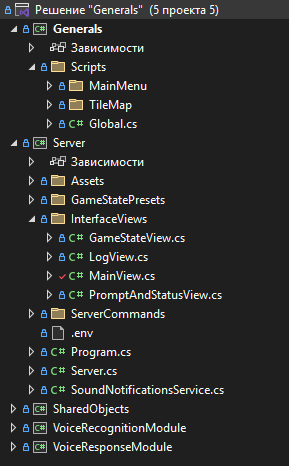
\includegraphics[height=0.75\textheight]{pictures/godot_fs.png}
\end{figure}
\pagebreak

\section*{ПРИЛОЖЕНИЕ Г}
\begin{figure}[H]
    \centering
    \caption{Файловая структура C\#-проекта на Citrus}\label{app2}
    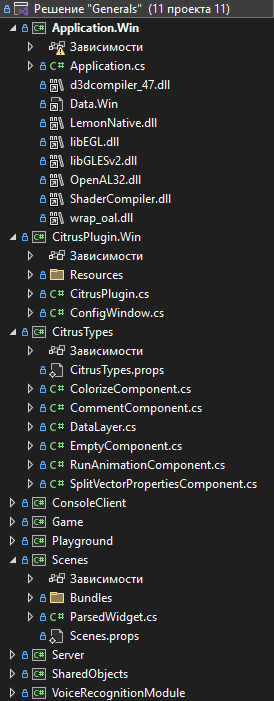
\includegraphics[height=0.85\textheight]{pictures/citrus_fs.png}
\end{figure}
\pagebreak

\section*{ПРИЛОЖЕНИЕ Д}
\begin{lstlisting}[caption=Цикл сражения юнитов]
    public void ProcessFight(GameState gs, TimeSpan timeDelta)
    {
        lock (_lock)
        {
            List<BaseUnit> p1Units = [];
            List<BaseUnit> p2Units = [];
            List<int> deadUnitsIds = [];
            foreach (int unitId in CellUnitIds)
            {
                var curUnit = gs.GetUnitById(unitId);
                if (curUnit.PlayerId == 0)
                    p1Units.Add(curUnit);
                else
                    p2Units.Add(curUnit);
            }
            AttackEnemies(p1Units, p2Units, deadUnitsIds, timeDelta);
            foreach (var deadId in deadUnitsIds)
            {
                RemoveCellUnit(deadId);
                gs.RemoveUnit(deadId);
            }
        }
    }
    private void AttackEnemies(List<BaseUnit> allies, List<BaseUnit> enemies, List<int> dead, TimeSpan timeDelta)
    {
        int p = 0;
        for (int i = 0; p < enemies.Count && i < allies.Count; i++)
        {
            var curUnit = allies[i];
            var curEnemy = enemies[p];
            if (curUnit.OnCooldown)
            {
                curUnit.Elapsed += timeDelta;
                if (curUnit.Elapsed >= TimeSpan.FromSeconds(curUnit.AttackSpeed))
                {
                    curUnit.Elapsed = TimeSpan.Zero;
                    curUnit.OnCooldown = false;
                }
            }
            else
            {
                curEnemy.Health -= curUnit.AttackDamage;
                curUnit.OnCooldown = true;
            }
    
            if (curEnemy.Health <= 0)
            {
                dead.Add(curEnemy.UnitId);
                p++;
            }
        }
    }
\end{lstlisting}\label{app4}
